\documentclass{beamer}
\usepackage[utf8]{inputenc}
\usetheme{Madrid}
\usecolortheme{default}
\usepackage{amsmath,amssymb,amsfonts,amsthm}
\usepackage{txfonts}
\usepackage{tkz-euclide}
\usepackage{listings}
\usepackage{adjustbox}
\usepackage{array}
\usepackage{tabularx}
\usepackage{gvv}
\usepackage{lmodern}
\usepackage{circuitikz}
\usepackage{tikz}
\usepackage{graphicx}
\setbeamertemplate{page number in head/foot}[totalframenumber]
\usepackage{tcolorbox}
\tcbuselibrary{minted,breakable,xparse,skins}
\definecolor{bg}{gray}{0.95}
\DeclareTCBListing{mintedbox}{O{}m!O{}}{%
  breakable=true,
  listing engine=minted,
  listing only,
  minted language=#2,
  minted style=default,
  minted options={%
    linenos,
    gobble=0,
    breaklines=true,
    breakafter=,,
    fontsize=\small,
    numbersep=8pt,
    #1},
  boxsep=0pt,
  left skip=0pt,
  right skip=0pt,
  left=25pt,
  right=0pt,
  top=3pt,
  bottom=3pt,
  arc=5pt,
  leftrule=0pt,
  rightrule=0pt,
  bottomrule=2pt,
  toprule=2pt,
  colback=bg,
  colframe=orange!70,
  enhanced,
  overlay={%
    \begin{tcbclipinterior}
    \fill[orange!20!white] (frame.south west) rectangle ([xshift=20pt]frame.north west);
    \end{tcbclipinterior}},
  #3,
}

\title{2.7.17 Solution}
\date{September 19, 2025}
\author{Aditya Mishra - EE25BTECH11005}

\begin{document}

\frame{\titlepage}

\begin{frame}{Problem}
Show that the points \(\vec{A} = 2\hat{i} - \hat{j} + \hat{k}\), \(\vec{B} = \hat{i} - 3\hat{j} - 5\hat{k}\), and \(\vec{C} = 3\hat{i} - 4\hat{j} - 4\hat{k}\) are vertices of a right-angled triangle. Find the area of the triangle.
\end{frame}

\begin{frame}{Given Vectors}
\[
\vec{A} = \myvec{2 \\ -1 \\ 1}, \quad
\vec{B} = \myvec{1 \\ -3 \\ -5}, \quad
\vec{C} = \myvec{3 \\ -4 \\ -4}
\]
\end{frame}

\begin{frame}{Check Right Angle at \(\vec{A}\)}
Side vectors:
\[
\vec{B} - \vec{A} = \myvec{-1 \\ -2 \\ -6}, \quad
\vec{C} - \vec{A} = \myvec{1 \\ -3 \\ -5}
\]

Dot product:
\[
(\vec{B} - \vec{A})^\top (\vec{C} - \vec{A}) = -1 + 6 + 30 = 35 \neq 0
\]

No right angle at \( \vec{A} \).
\end{frame}

\begin{frame}{Check Right Angle at \(\vec{B}\)}
Side vectors:
\[
\vec{A} - \vec{B} = \myvec{1 \\ 2 \\ 6}, \quad
\vec{C} - \vec{B} = \myvec{2 \\ -1 \\ 1}
\]

Dot product:
\[
(\vec{A} - \vec{B})^\top (\vec{C} - \vec{B}) = 2 - 2 + 6 = 6 \neq 0
\]

No right angle at \( \vec{B} \).
\end{frame}

\begin{frame}{Right Angle at \(\vec{C}\)}
Side vectors:
\[
\vec{A} - \vec{C} = \myvec{-1 \\ 3 \\ 5}, \quad
\vec{B} - \vec{C} = \myvec{-2 \\ 1 \\ -1}
\]

Dot product:
\[
(\vec{A} - \vec{C})^\top (\vec{B} - \vec{C}) = 0
\]

Right angle at \( \vec{C} \).
\end{frame}

\begin{frame}{Area Calculation}
\begin{center}
\[
\text{Area} = \frac{1}{2} \left\| (\vec{A} - \vec{C}) \times (\vec{B} - \vec{C}) \right\| 
= \frac{1}{2} \left\|
\myvec{
\left|
\begin{matrix}
3 & 1 \\
5 & -1
\end{matrix}
\right|
\\
\left|
\begin{matrix}
5 & -1 \\
-1 & -2
\end{matrix}
\right|
\\
\left|
\begin{matrix}
-1 & 3 \\
-2 & 1
\end{matrix}
\right|
}
\right\| 
= \frac{1}{2} \sqrt{210}.
\]
\end{center}

\end{frame}
\begin{frame}{Plot}
\begin{figure}
    \centering
    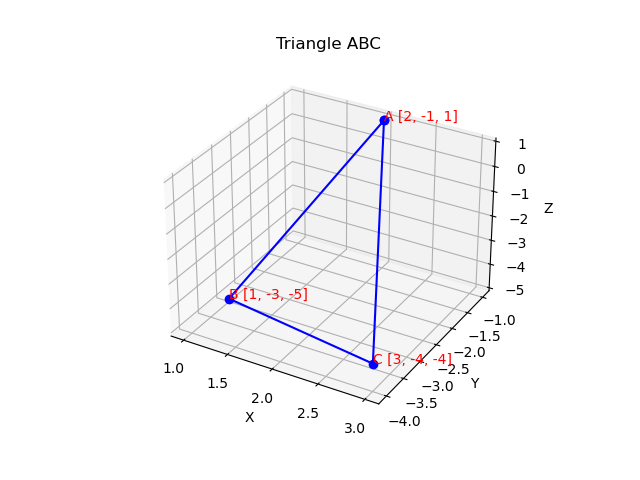
\includegraphics[width=0.8\columnwidth]{Figs/Figure_1.png}
    \caption{Plot}
    \label{fig:placeholder}
\end{figure}
\end{frame}
\begin{frame}{Codes}
	\centering
	For Codes refer to the URL given below:
	\url{https://github.com/Aditya-Mishra11005/ee1030-2025/tree/main/ee25btech11005/matgeo/2.7.17/Codes}
\end{frame}
\end{document}

